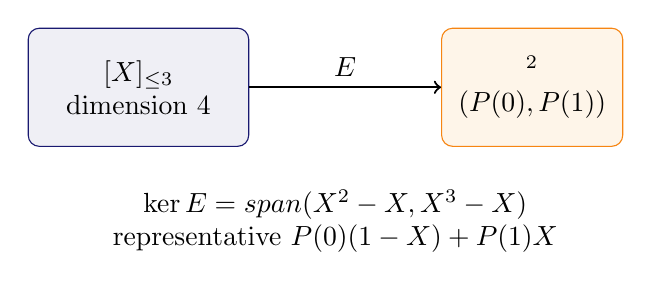
\begin{tikzpicture}[x=1cm,y=1cm]
\node[draw=MidnightBlue,fill=MidnightBlue!7,rounded corners,align=center,minimum width=2.8cm,minimum height=1.5cm] (v) at (0,0) {$\R[X]_{\le3}$\\dimension $4$};
\node[draw=BurntOrange,fill=BurntOrange!7,rounded corners,align=center,minimum width=2.3cm,minimum height=1.5cm] (q) at (5,0) {$\R^2$\\$(P(0),P(1))$};
\draw[->,thick] (v)--(q) node[midway,above] {$E$};
\node[align=center] at (2.5,-1.7) {$\ker E=\operatorname{span}(X^2-X,X^3-X)$\\representative $P(0)(1-X)+P(1)X$};
\end{tikzpicture}
